%%
% Please see https://bitbucket.org/rivanvx/beamer/wiki/Home for obtaining beamer.
%%
\documentclass{beamer}

\usepackage[utf8]{inputenc}
\usepackage[italian]{babel}
\usepackage{graphicx}
\usepackage{montserrat}

\usetheme{revas}

\title{Authentication in Revas}

\begin{document}

\frame{\titlepage}

\begin{frame}
	\frametitle{What is Authentication?}
	
	Authentication is the process of determining whether someone or something is, in fact, who or what it declares itself to be.
\end{frame}

\begin{frame}
	\frametitle{Revas uses token based authentication}
	
	Token-based authentication is a protocol which allows users to verify their identity, and in return receive a unique access token.  \newline
	During the life of the token, users then access the website the token has been issued for, rather than having to re-enter credentials each time they go back to the same webpage.  \newline
	Auth tokens work like a stamped ticket. The user retains access as long as the token remains valid.
\end{frame}

\begin{frame}
	\frametitle{What will we see}
	
	\begin{itemize}
		\item How to protect tokens
		\item How to represent tokens
		\item How to obtain tokens
	\end{itemize}
\end{frame}

\begin{frame}
	\frametitle{How to pass information securely?}
	
	{\footnotesize \textbf{\textcolor{revassecondary}{Cryptography}}}
	
	Ancient practice and study of techniques for secure communication in the presence of third parties called adversaries.  \newline
	Very used in military communications.
	
\end{frame}

\begin{frame}
	\frametitle{Common cryptographic algorithms}
	
	{\footnotesize \textbf{\textcolor{revassecondary}{Symmetric encryption}}}
	
	The simplest and best-known encryption technique. \textbf{It uses one key for both encryption and decryption.} \newline
	{\small The plaintext is encrypted using a key, and the same key is used at the receiving end to decrypt the received ciphertext. The host in the communication process would have \textbf{received the key through external means.}} 
	
	 {\footnotesize \textbf{\textcolor{revassecondary}{Adavantages}}}
	\begin{itemize}	
		\item Fast
		\item Easy
	\end{itemize}	
	
	 {\footnotesize \textbf{\textcolor{revassecondary}{Disadvantages}}}
	\begin{itemize}	
		\item Hard to distribute key
		\item If key is leaked, you have to replace it and tell everyone the new key again
		\item Do not have proof of who sent the message
	\end{itemize}	
\end{frame}

\begin{frame}
	\frametitle{Symmetric encryption}

	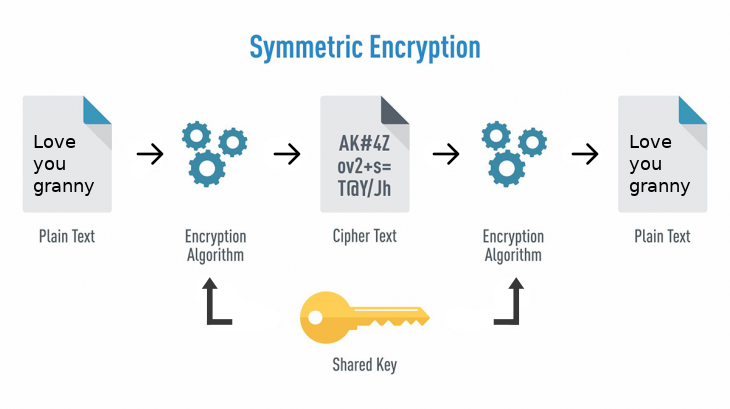
\includegraphics[width=\textwidth]{./resources/symmetric_encryption.png}
	
\end{frame}

\begin{frame}
	\frametitle{Common cryptographic algorithms}
	
	{\footnotesize \textbf{\textcolor{revassecondary}{Asymmetric encryption}}}
	
	More secure than symmetric encryption as it uses two keys for the process.
	The public key used for encryption is available to everyone but the private key is not disclosed.
	When a message is encrypted using a public key, it can only be decrypted using a private key. However, when a message is encrypted using a private key, it can be decrypted using a public key. \newline
	{\footnotesize \textbf{\textcolor{revassecondary}{Adavantages}}}: 
	\begin{itemize}	
		\item Public key can be safely shared
		\item Proof that the message was signed by whoever is in possession of the private key 
	\end{itemize}	
	
	 {\footnotesize \textbf{\textcolor{revassecondary}{Disadvantages}}}: 
	\begin{itemize}	
		\item Slow
	\end{itemize}
\end{frame}

\begin{frame}
	\frametitle{Asymmetric encryption}
	
	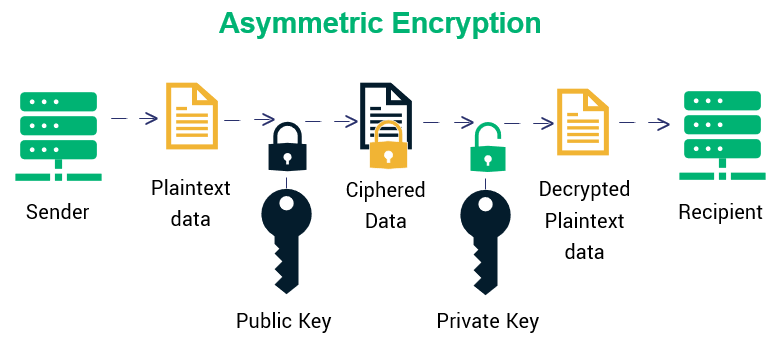
\includegraphics[width=\textwidth]{./resources/asymmetric_encryption.png}
	
\end{frame}

\begin{frame}
	\frametitle{Revas Tokens}\ \newline
	
	Token can be signed and/or encrypted, in Revas it's sufficient to digitally signed them.
	Cryptograhy is used to digitally sign them.
\end{frame}

\begin{frame}
	\frametitle{Digital Signature}\ \newline
	
	A digital signature is a mathematical scheme for verifying the authenticity of digital messages or documents. A valid digital signature, where the prerequisites are satisfied, gives a recipient very strong reason to believe that the message was created by a known sender (authentication), and that the message was not altered in transit (integrity)

\end{frame}

\begin{frame}
	\frametitle{Signing algorithms}\ \newline
	
HS256 (HMAC with SHA-256): A symmetric algorithm
RS256 (RSA Signature with SHA-256): An asymmetric algorithm
\end{frame}

\begin{frame}
	\frametitle{Most secure signing algorithm}\ \newline
	
The most secure practice, is to use RS256 because:

\begin{itemize}	
		\item With RS256, you are sure that only the holder of the private key (Auth0) can sign tokens, while anyone can check if the token is valid using the public key.
		\item With RS256, if the private key is compromised, you can implement key rotation without having to re-deploy your application or API with the new secret (which you would have to do if using HS256).
	\end{itemize}	

\end{frame}

\begin{frame}
	\frametitle{Access Token in JWT format}\ \newline
	
	JSON Web Token (JWT) is an open standard (RFC 7519) that defines a compact and self-contained way for securely transmitting information between parties as a JSON object. This information can be verified and trusted because it is digitally signed. JWTs can be signed using a secret (with the HMAC algorithm) or a public/private key pair using RSA or ECDSA.
\end{frame}

\begin{frame}
	\frametitle{JWT structure}\ \newline
	
	Structure
	\begin{itemize}	
		 \item Header
		 \item Paylaod
		 \item Signature
	\end{itemize}

\end{frame}

\begin{frame}
	\frametitle{JWT structure: Header }\ \newline
	
	The header typically consists of two parts: the type of the token, which is JWT, and the signing algorithm being used, such as HMAC SHA256 or RSA. It is Base64Url encoded.

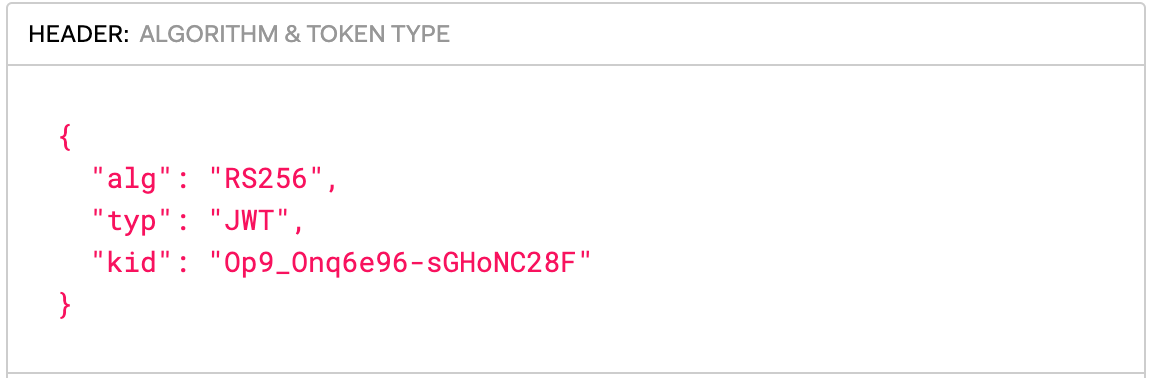
\includegraphics[width=\textwidth]{./resources/revas-header}

\end{frame}

\begin{frame}
	\frametitle{JWT structure: Payload }\ \newline
	 Contains the claims which are statements about an entity (typically, the user) and additional data. There are three types of claims: registered, public, and private claims.
	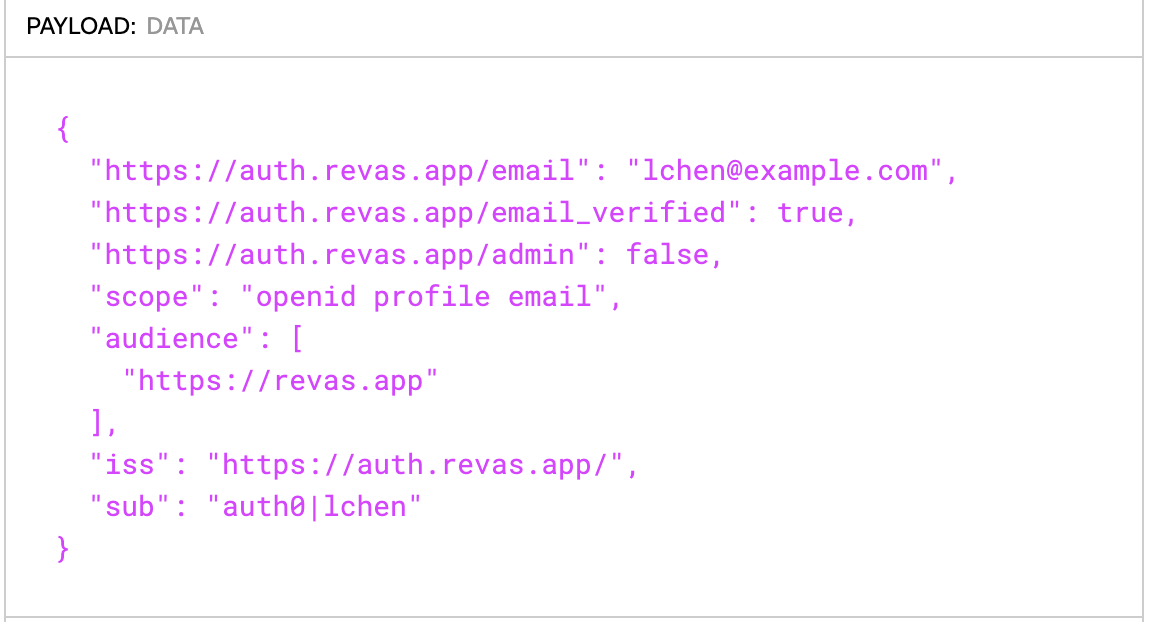
\includegraphics[width=\textwidth]{./resources/revas-payload}

\end{frame}

\begin{frame}
	\frametitle{JWT structure: Signature}\ \newline
	
	The purpose of the signature is to protect/validate the integrity of the data (e.g. the user id) that the server sends and eventually gets back.\newline
	In the case of tokens signed with a private key, it can also verify that the sender of the JWT is who it says it is.
	
\end{frame}

\begin{frame}
	\frametitle{How to sign tokens}\ \newline
	
	Symmetric key example
	\begin{itemize}	
		\item What we do is we take the  \textbf{Header}, the \textbf{Payload} and we add also a \textbf{secret password}, and then we hash everything together.
		\item The result of that function can only be reproduced by someone in possession of all the above 3 things.
	\end{itemize}
\end{frame}

\begin{frame}
	\frametitle{How to validate tokens}\ \newline
	
	Symmetric key example
	\begin{itemize}	
		\item To check the signature we simply take the JWT header + the payload and hash it together with the password.
		\item And if we get back the same hash as in the signature it means that the token must be valid, because only someone with the password could have come up with that signature
		\end{itemize}
\end{frame}

\begin{frame}
	\frametitle{Encryption and Hashing}\ \newline
	
	Encryption is a two-way function; what is encrypted can be decrypted with the proper key. Reversible key systems can be used for confidentiality, integrity, and non-repudiation. \newline \newline
	Hashing, however, is a one-way function that scrambles plain text to produce a unique message digest. Irreversible key systems can only be used for integrity and non-repudiation.  \newline \newline
	Signature-based communication relies on a one-way hashing function.
\end{frame}

\begin{frame}
	\frametitle{JWT: self-contained}\ \newline

The key property of JWTs is that in order to confirm if they are valid we only need to look at the token itself.

We don't have to contact a third-party service or keep JWTs in-memory between requests to confirm that the claim they carry is valid.
The signed JWT acts effectively as a temporary user credential, that replaces the permanent credential which is the username and password combination.
\end{frame}

\begin{frame}
	\frametitle{JWT best practices}\ \newline
	
	\begin{itemize}	
		\item Use secure connection when transferring tokens;
		\item Never transfer users’ sensitive data in the tokens;
		\item Limit JWT lifespan and use “refresh tokens” mechanism;
		\item Use long key phrases (Mining the key for signature symmetric algorithm);
		\item Keep a white list of authorised signature algorithms on the application side;
		\item Work, ideally, with one signature algorithm only;
		\item Choose well-known and reliable libraries for JWT operation;
		\item Always validate and sanitise the data received from users.
	\end{itemize}	

\end{frame}

\begin{frame}
	\frametitle{Where to store JWT?}\ \newline
	
	It is not recommended to store the JWT in the browser local storage:

It will remain if the user closes the browser so the session can be restored until the JWT expires.
Any JavaScript code on your page can access local storage: it has no data protection whatsoever.
It can’t be used by web workers
Storing JWT in session cookie may be the solution
\end{frame}

\begin{frame}
	\frametitle{OAuth2.0}
	
	Is a security standard that defines an \textbf{authorization} framework to allow access to specific information without sharing passwords.  \newline
\end{frame}

\begin{frame}
	\frametitle{OAuth Roles}\
	
	\begin{itemize}	
		\item  {\footnotesize \textbf{\textcolor{revassecondary}{Resource Owner}}}: Entity that can grant access to a protected resource. Typically, this is the end-user. (Mike)
		\item  {\footnotesize \textbf{\textcolor{revassecondary}{Client}}}: Application requesting access to a protected resource on behalf of the Resource Owner. (Revas Platform)
		\item  {\footnotesize \textbf{\textcolor{revassecondary}{Authorization Server}}}: Server that authenticates the Resource Owner and issues access tokens after getting proper authorization. For Revas is, Auth0.
		\item   {\footnotesize \textbf{\textcolor{revassecondary}{Resource Server}}} : Server hosting the protected resources. This is the API you want to access.  (Revas API)
	\end{itemize}	
\end{frame}

\begin{frame}
	\frametitle{OAuth Scopes}\
	
	They are used to specify exactly the reason for which access to resources may be granted.	
\end{frame}

\begin{frame}
	\frametitle{OAuth Access Tokens}\
	
	An Access Token is a piece of data that represents the authorization to access resources on behalf of the end-user.\ \newline
	Refresh tokens are used to obtain a renewed access token without having to re-authenticate the user. They are better than long lived access token because they can be revoked in case on misuse.
\end{frame}

\begin{frame}
	\frametitle{OAuth Flows}\
	OAuth defines \textbf{flows}, also called grants, which are mechanisms for a client to get credentials (an access token) from an Authorization Server to access a protected resource.
	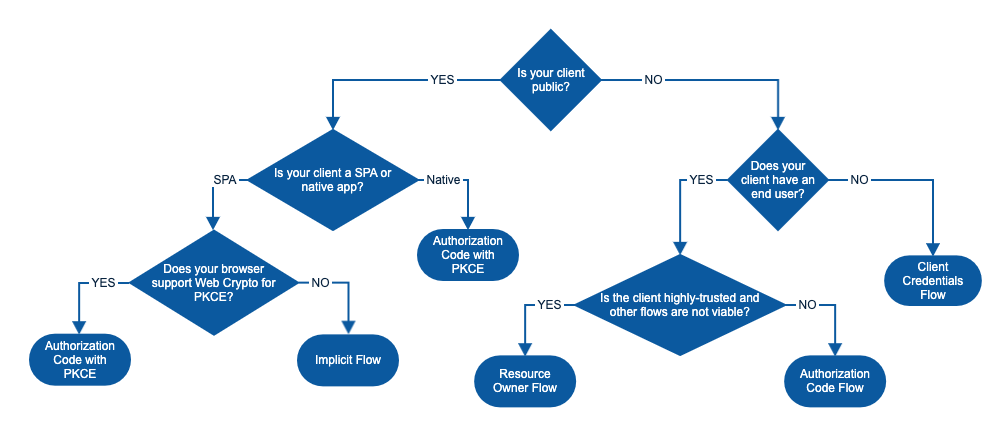
\includegraphics[width=\textwidth]{./resources/oauth_grant_flowchart.png}	
\end{frame}

\begin{frame}
	\frametitle{Authorization Code Flow}\
	
	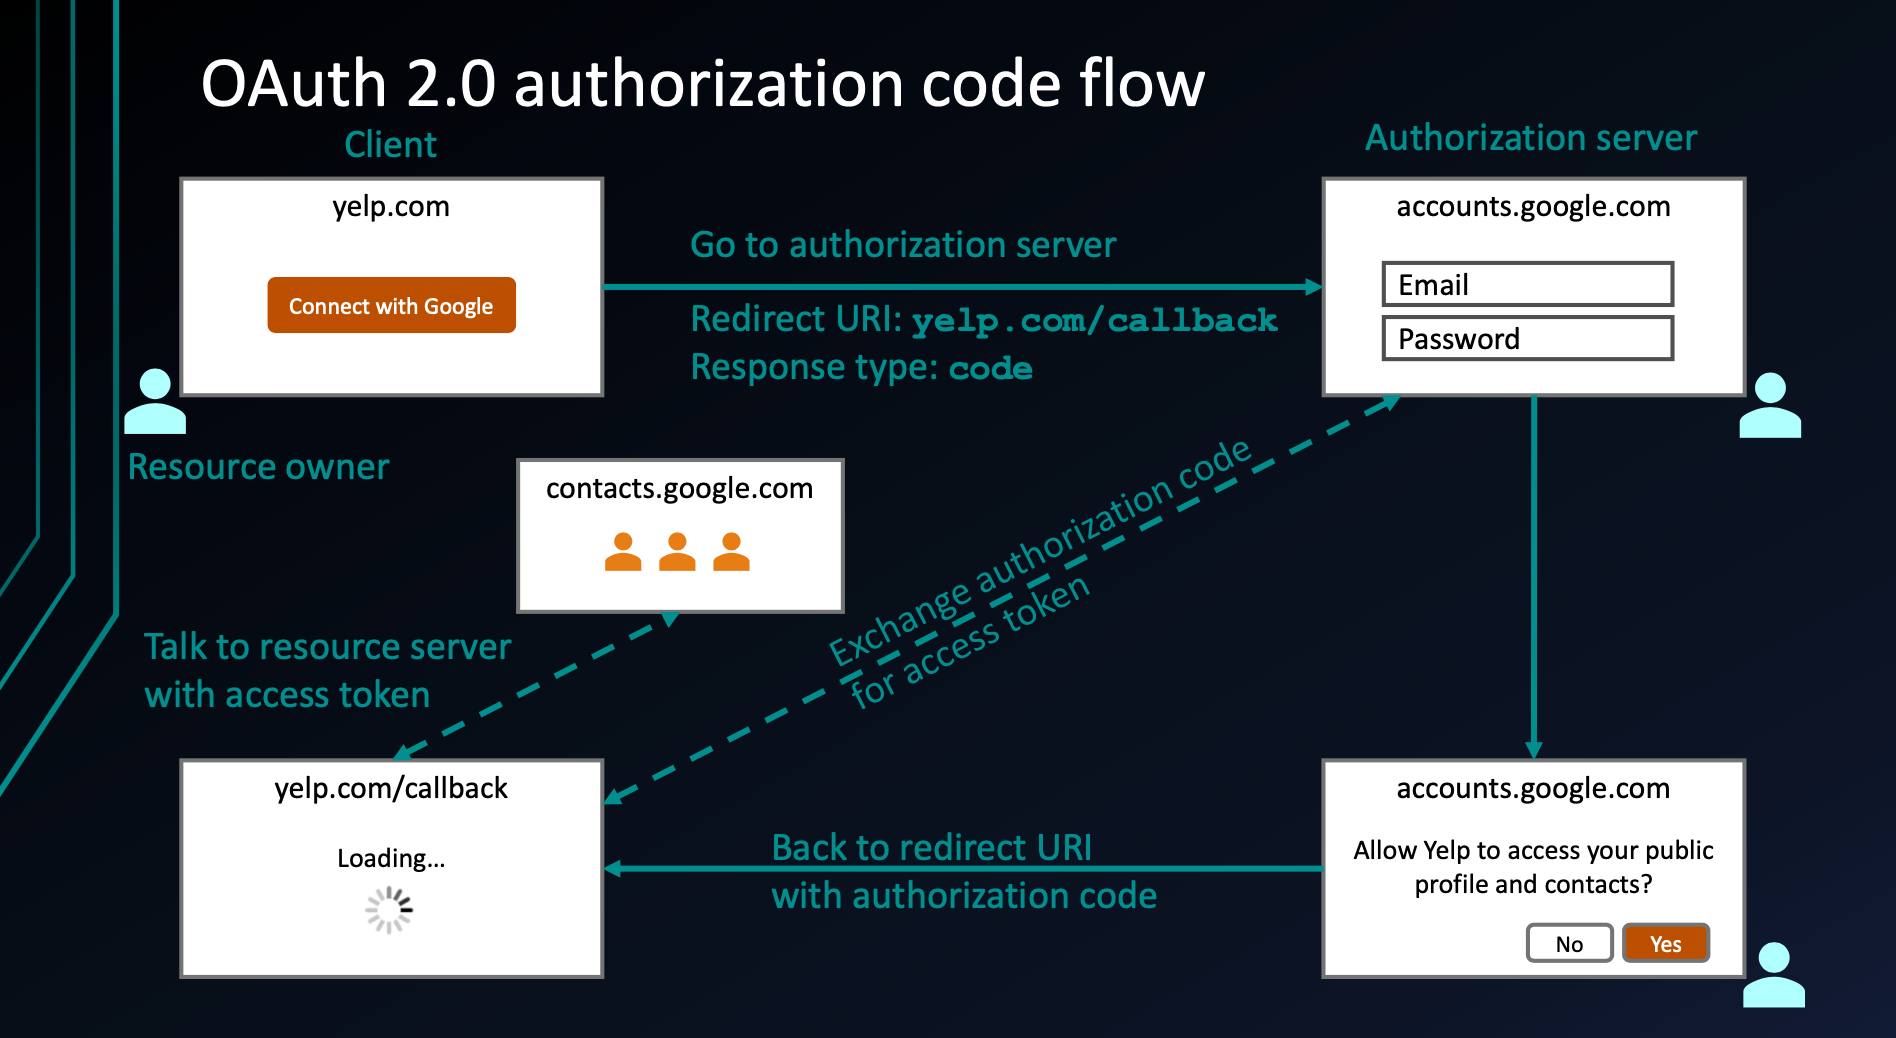
\includegraphics[width=\textwidth]{./resources/authorization-code-flow.png}
	
\end{frame}



\begin{frame}
	\frametitle{PKCE: Proof key for code exchange}\ \newline

	All the principle of code flow still applies. The PKCE makes this more safe for native and web applications (public clients) by generating a code exchange key, that ensures that the authorization request and the token request is done by the  \textbf{same client} (aka not intercepted by a man in the middle). Because web applications can’t store secrets, PKCE allows for creating a secret dynamically at the beginning of the authorization flow as a contrast to the static secret in code flow (can only be used for private/server clients).
	
\end{frame}

\begin{frame}
	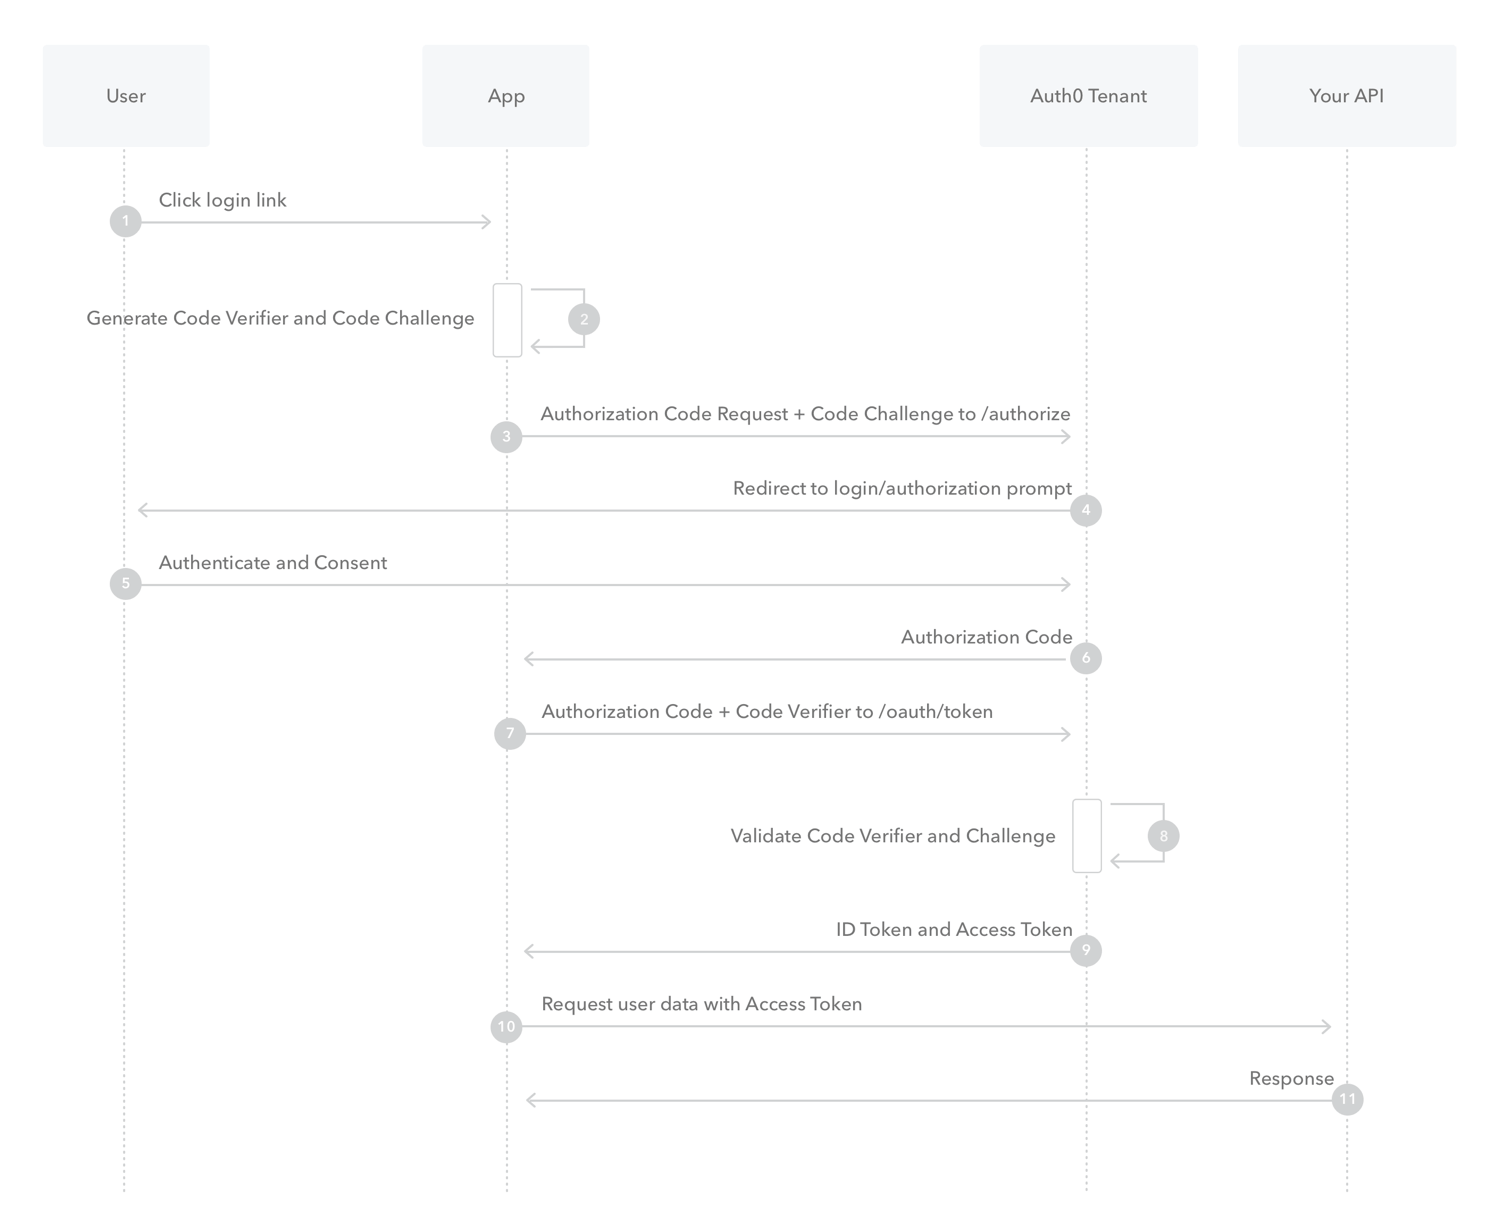
\includegraphics[width=\textwidth]{./resources/pkce-flow.png}
	
\end{frame}

\begin{frame}
	\frametitle{OpenID Connect for authentication}\ \newline
	
	In the world of consent and authorization, identity was missing.
	OIDC adds
	\begin{itemize}	
		 \item ID Token
		 \item UserInfo endpoint for getting more user information
		 \item Standard set of scopes
		 \item Standardized implementation
	\end{itemize}	
	The OIDC looks like OAuth the only difference are in the initial request, a specific scope of openid is used and in the final exchange the client receives both an access token and an ID token. 
\end{frame}

\begin{frame}
	\frametitle{Thanks to OAuth and OIDC}
	
	\begin{itemize}	
		 \item Authorizing third party services to access information in another service.
			For example letting Facebook post your wonderful score on Candy Crush.
	
		 \item Single Sign-on (SSO) occurs when a user logs in to one application and is then signed in to other applications automatically, regardless of the platform.
			For example, if you log in to a Google service such as Gmail, you are automatically authenticated to YouTube, AdSense, Google Analytics, and other Google apps.
	
		 \item Sign-in to other service using an Identity Providers without the need to create another account.
	\end{itemize}	
\end{frame}

\begin{frame}
	\frametitle{Identity Provider}
	An identity provider is a system entity that creates, maintains, and manages identity information for principals and also provides authentication services to relying applications. \newline
	A single, consistent identity that can be used across platforms, applications and networks is called a federated identity. 
	
	Most used Identity Providers
	\begin{itemize}	
		\item Google
		\item Facebook
		\item Instagram
		\item Fitbit.
		\item Microsoft
\end{itemize}	
	
\end{frame}

\begin{frame}
	\frametitle{How do OpenID providers authenticate users?}
	
	OpenID Connect leaves this entirely up to the particular IdP. Implementors may use any method for authenticating users, or combine two methods for stronger security (2FA).
	\begin{itemize}	
 		\item Username / password
		 \item Hardware tokens
		 \item SMS confirmation
		 \item Biometrics
		 \item Etc.
	\end{itemize}
\end{frame}

\begin{frame}
 \frametitle{To summarize}
 
 Revas uses
 \begin{itemize} 
   \item Auth0 as Identity Provider delegating most of the authentication managment
   \item RSA with SHA-256 to sign tokens which uses the asymmetric algoritm, the most secure one
   \item PCKE flow to obtain the access token, most secure flow for now...
   \item Passwordless to handle user credentials
 \end{itemize}
\end{frame}

\end{document}
